\documentclass[11pt,a4paper]{article}
\usepackage[utf8]{inputenc}
\usepackage[T1]{fontenc}
\usepackage{graphicx}
\usepackage{hyperref}
\usepackage{listings}
\usepackage{xcolor}
\usepackage{geometry}
\usepackage{amsmath}
\usepackage{booktabs}
\usepackage{pdfpages} % Adding package for PDF inclusion

\geometry{margin=2.5cm}

\title{SATIM Challenge: Policy Compliance Analysis System}
\author{Technical Report}
\date{\today}

\begin{document}

\maketitle

\begin{abstract}
This technical report presents the SATIM Challenge project, a sophisticated policy compliance analysis system that leverages artificial intelligence to compare internal policies against global regulations. The system utilizes advanced natural language processing techniques, vector databases, and large language models to provide comprehensive policy analysis and recommendations. This report details the system architecture, implementation, and technical specifications.
\end{abstract}

\section{Introduction}
The SATIM Challenge project addresses the critical need for automated policy compliance analysis in organizations. The system provides a robust solution for comparing internal policies against global regulations, identifying gaps, and suggesting improvements. This automated approach significantly reduces the time and resources required for manual policy analysis while ensuring comprehensive coverage of regulatory requirements.

\section{System Architecture}
\subsection{Overview}
The system is built using a modern web application architecture with the following key components:
\begin{itemize}
    \item Flask-based web server
    \item Policy Analyzer engine
    \item Vector database for policy storage
    \item OpenRouter API integration for LLM capabilities
    \item File processing system
\end{itemize}

\subsection{Core Components}
\subsubsection{Web Application (app.py)}
The web application serves as the primary interface for users to interact with the system. Key features include:
\begin{itemize}
    \item File upload handling for PDF documents
    \item Text-based policy input
    \item Multi-language support (English and French)
    \item Automatic file cleanup system
    \item Error handling and logging
\end{itemize}

\subsubsection{Policy Analyzer (policy\_analyzer.py)}
The Policy Analyzer is the core engine that performs the policy analysis. It implements:
\begin{itemize}
    \item Vector database initialization and management
    \item Policy comparison algorithms
    \item LLM integration through OpenRouter API
    \item Structured analysis report generation
\end{itemize}

\section{Technical Implementation}
\subsection{Vector Database Integration}
The system utilizes vector databases to store and retrieve policy documents efficiently. The implementation includes:
\begin{itemize}
    \item Separate databases for internal and global policies
    \item Document loading and processing
    \item Similarity search functionality
    \item Efficient document retrieval
\end{itemize}

\subsection{Language Model Integration}
The system integrates with Mistral-7B through the OpenRouter API to provide intelligent policy analysis. Key features include:
\begin{itemize}
    \item Custom prompt templates for different languages
    \item Structured analysis output
    \item Error handling and fallback mechanisms
\end{itemize}

\section{Features and Capabilities}
\subsection{Policy Analysis}
The system provides comprehensive policy analysis with the following outputs:
\begin{itemize}
    \item Missing policies identification
    \item Implemented policies review
    \item Improvement suggestions
    \item Best practices recommendations
\end{itemize}

\subsection{Multi-language Support}
The system supports both English and French languages for:
\begin{itemize}
    \item User interface
    \item Policy analysis
    \item Report generation
\end{itemize}

\section{Security and Performance}
\subsection{Security Measures}
\begin{itemize}
    \item Secure file handling
    \item API key management
    \item Input validation
    \item File size restrictions
\end{itemize}

\subsection{Performance Optimizations}
\begin{itemize}
    \item Automatic file cleanup
    \item Efficient vector search
    \item Caching mechanisms
    \item Error handling and logging
\end{itemize}

\section{Technical Requirements}
\subsection{System Requirements}
\begin{itemize}
    \item Python 3.x
    \item Flask web framework
    \item Vector database storage
    \item OpenRouter API access
\end{itemize}

\subsection{Dependencies}
Key Python packages required:
\begin{itemize}
    \item Flask
    \item LangChain
    \item PyPDF2
    \item Requests
    \item Vector database libraries
\end{itemize}

\section{Solution Structure}
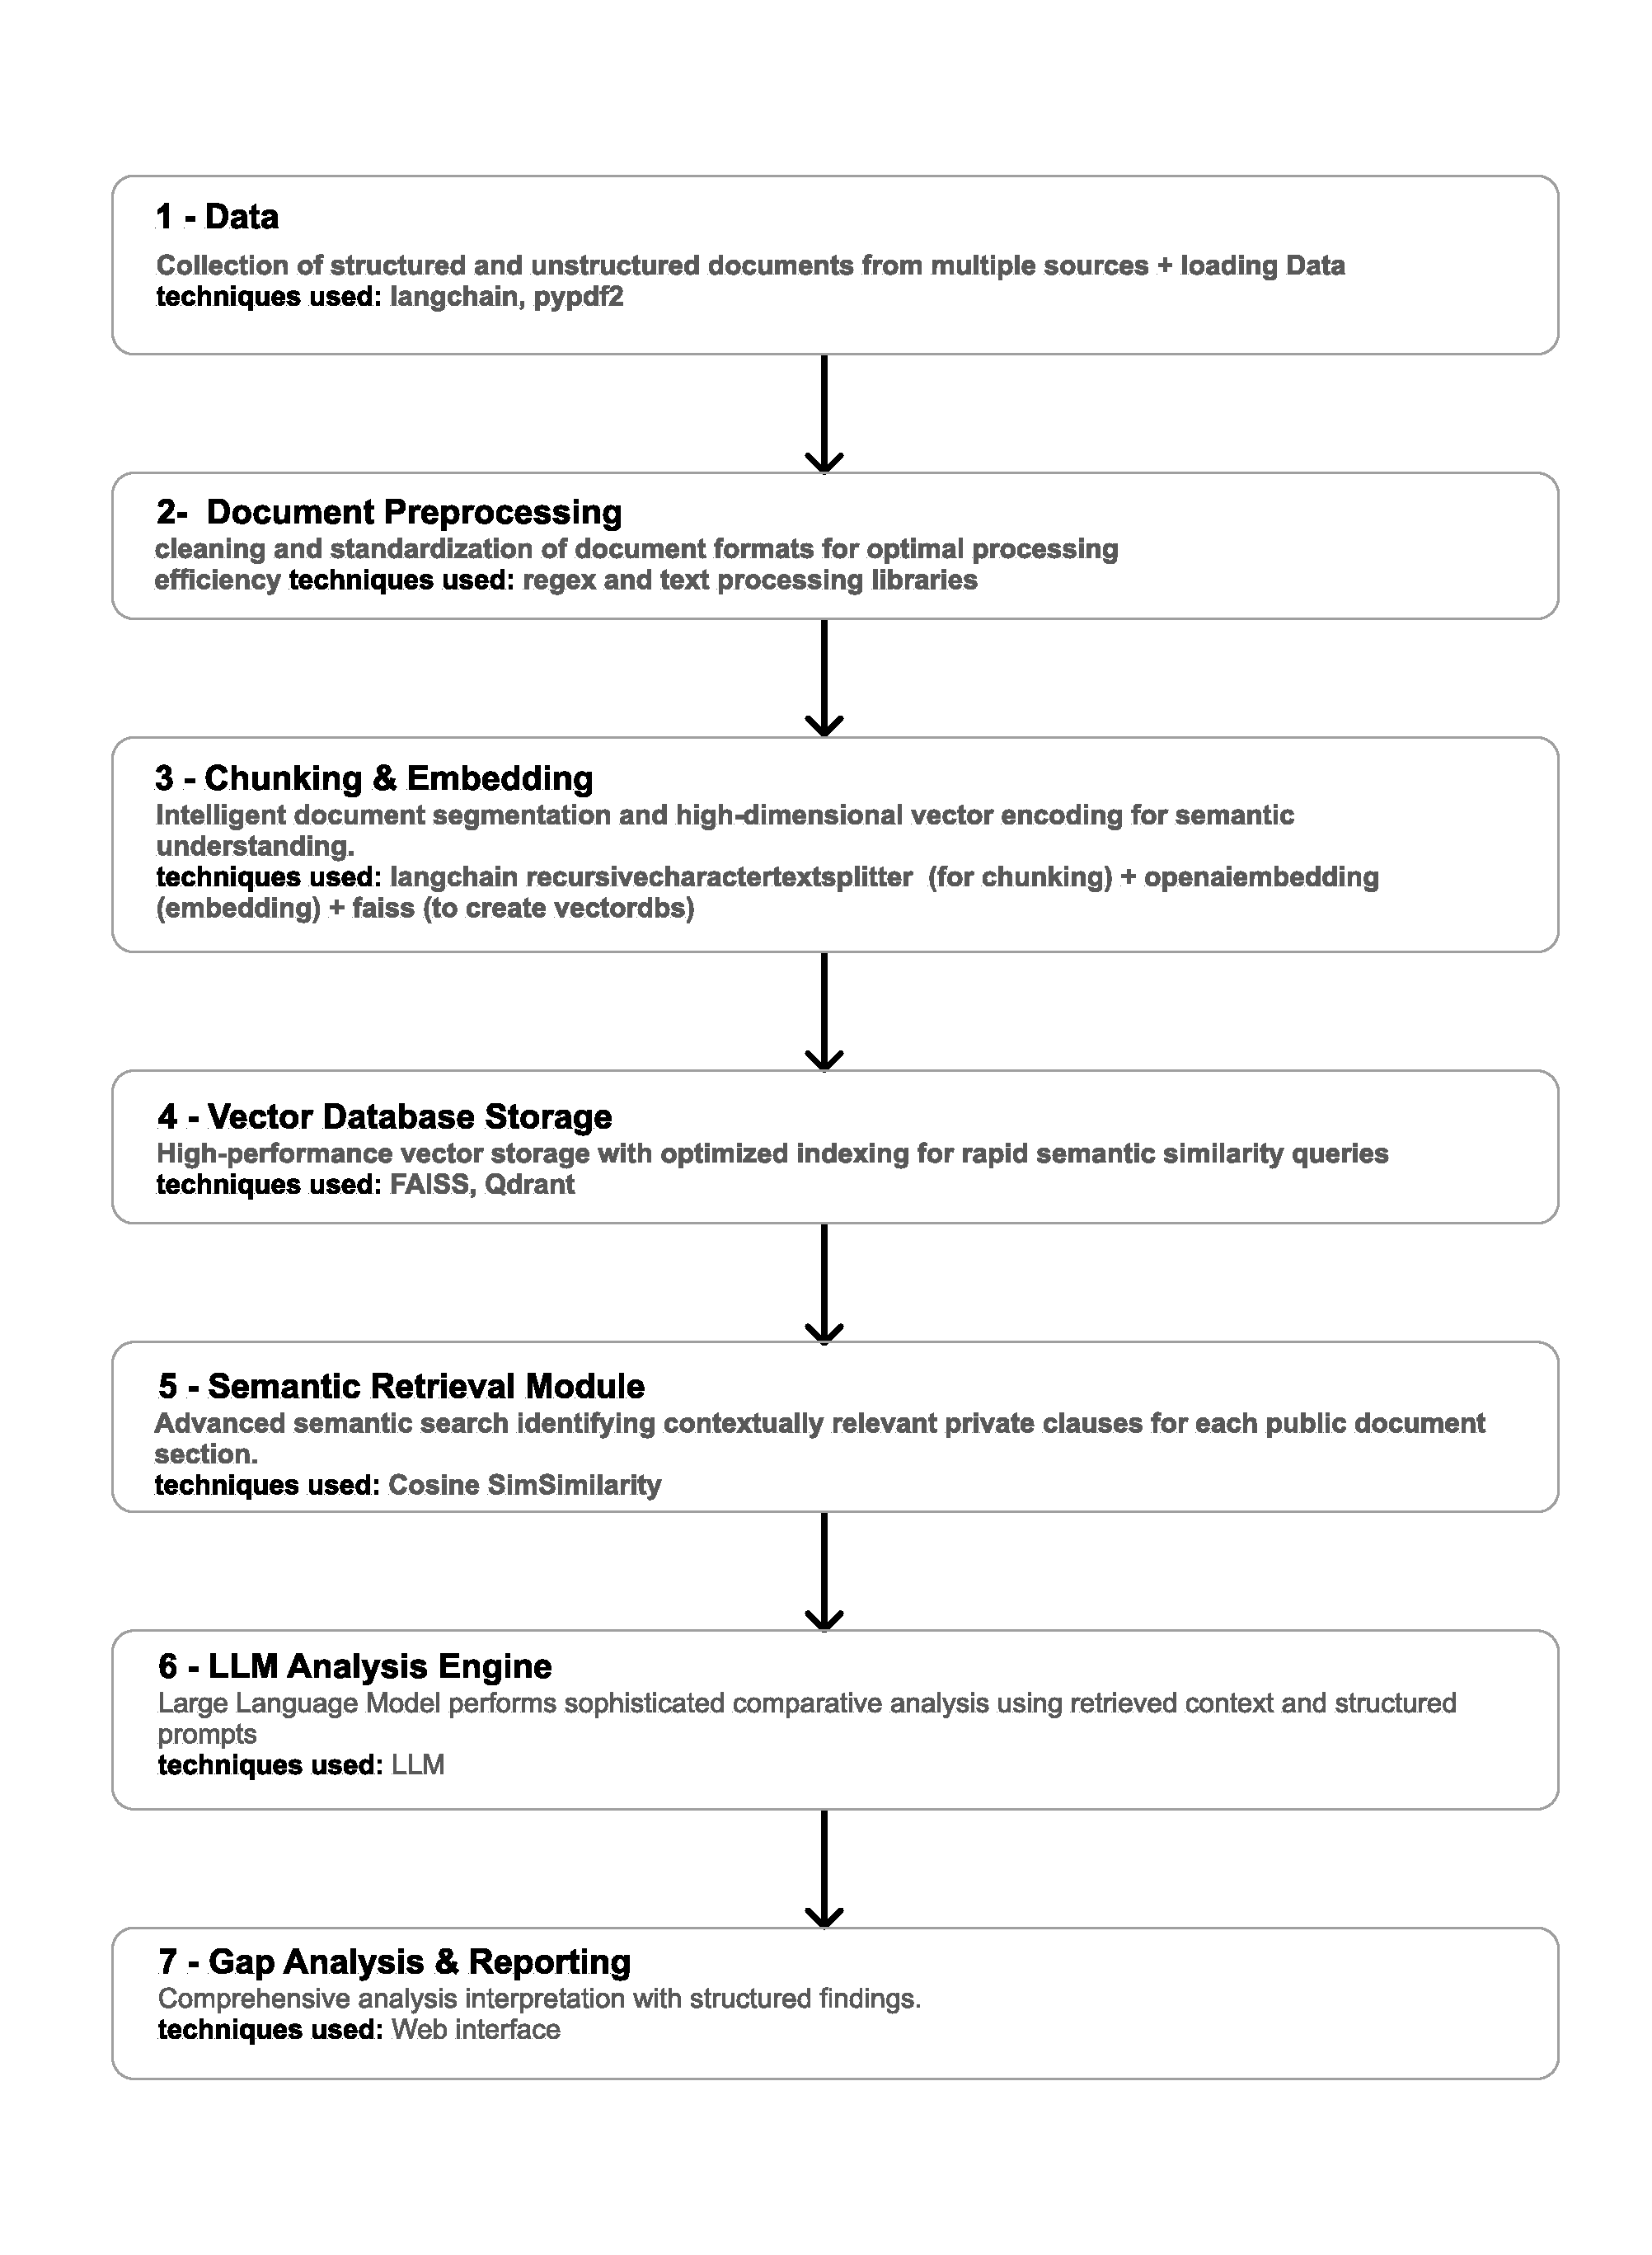
\includepdf[pages=-]{Solution Structure.pdf}

\section{Use Case Analysis}
\subsection{Overview}
The system includes a dedicated use case analysis feature that allows users to evaluate specific scenarios against internal policies. This feature supports both CIS v8 controls and custom use cases, providing a comprehensive analysis of policy compliance and implementation status.

\subsection{Key Features}
\begin{itemize}
    \item CIS v8 Control Integration
    \begin{itemize}
        \item Pre-defined set of CIS v8 controls
        \item Organized into Basic, Foundational, and Organizational categories
        \item Easy selection through dropdown interface
    \end{itemize}
    \item Custom Use Case Support
    \begin{itemize}
        \item Ability to define custom use cases
        \item Flexible input format
        \item Comprehensive analysis against internal policies
    \end{itemize}
    \item Analysis Components
    \begin{itemize}
        \item Compliance Score (0-100\%)
        \item Risk Assessment
        \item Implementation Status
        \item Policy Coverage Analysis
    \end{itemize}
\end{itemize}

\subsection{Technical Implementation}
The use case analyzer leverages the same core components as the policy analyzer but with specialized prompts and analysis templates:
\begin{itemize}
    \item Vector database search for relevant policies
    \item Structured prompt templates for consistent analysis
    \item Multi-language support (English and French)
    \item Real-time analysis and reporting
\end{itemize}

\subsection{Analysis Process}
The use case analysis follows a systematic approach:
\begin{enumerate}
    \item Input Processing
    \begin{itemize}
        \item CIS control selection or custom use case input
        \item Language preference detection
    \end{itemize}
    \item Policy Matching
    \begin{itemize}
        \item Vector similarity search for relevant policies
        \item Context gathering from matching policies
    \end{itemize}
    \item Analysis Generation
    \begin{itemize}
        \item Compliance score calculation
        \item Risk assessment
        \item Implementation status evaluation
        \item Policy coverage analysis
    \end{itemize}
    \item Results Presentation
    \begin{itemize}
        \item Structured output format
        \item Visual representation of KPIs
        \item Detailed analysis sections
    \end{itemize}
\end{enumerate}

\section{Future Improvements}
Potential areas for enhancement include:
\begin{itemize}
    \item Integration with additional regulatory databases
    \item Advanced reporting features
\end{itemize}


\section{Conclusion}
The SATIM Challenge project demonstrates a robust and scalable solution for automated policy compliance analysis. The system's architecture and implementation provide a solid foundation for future enhancements and broader adoption in organizational settings.

% Adding appendix for solution structure
\appendix


\end{document}